\documentclass{beamer}
\usepackage{amsfonts,amsmath,oldgerm}
\usepackage{clrscode4e}
\usepackage{ctex}

\usetheme{sintef}

\newcommand{\testcolor}[1]{\colorbox{#1}{\textcolor{#1}{test}}~\texttt{#1}}

\usefonttheme{serif}

\titlebackground{images/background.png}

\newcommand{\hrefcol}[2]{\textcolor{cyan}{\href{#1}{#2}}}

\title{数据结构与算法\\ Data Structure and Algorithm}
\subtitle{Introduction}
\author{\href{mailto:zlp@upc.edu.cn}{ZHANG Luping}}
\date{\today}

\begin{document}

\maketitle

\section{课程介绍}

\begin{frame}{课程所处地位}


    \begin{itemize}
        \item \textbf{《数据结构与算法》}是信息管理专业的\textcolor{red}{核心基础课程}之一。
        \item 它为学生提供解决实际问题和优化信息系统的\textcolor{red}{关键工具和技术}。
        \item 该课程与其他信息管理科学相关课程(如《管理信息系统》、《面向对象程序设计》、《商务智能与数据挖掘》、《信息系统分析与设计》等)相互关联,\textcolor{red}{构建了信息管理专业的技术基础}。
    \end{itemize}
    \begin{figure}
        \centering
        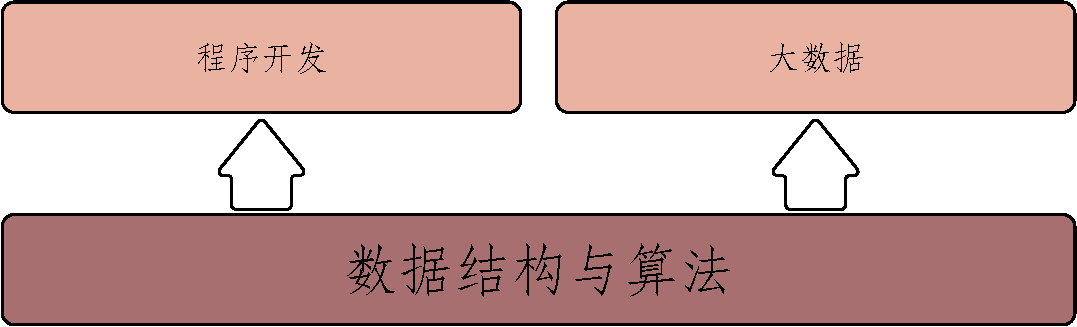
\includegraphics[width = 0.5\textwidth]{./images/import.pdf}
    \end{figure}


\end{frame}

\begin{frame}
    \frametitle{课程特征}

    \begin{itemize}
        \item \textbf{抽象性强}:数据结构与算法课程涉及到抽象的数据模型和算法设计,需要学生具备抽象思维和逻辑推理能力。
        \item \textbf{实践性强}:该课程注重实践操作和算法实现,学生需要通过编程实践来加深对数据结构和算法的理解和应用。
        \item \textbf{算法思维培养}:该课程强调培养学生的算法思维,即解决问题的思考方式和技巧,让学生具备分析、设计和优化算法的能力。
    \end{itemize}

\end{frame}

\begin{frame}
    \frametitle{主要讲授内容}

    \begin{itemize}
        \item 基本数据结构:包括数组、链表、栈、队列、树等常用数据结构的定义、实现和操作。
        \item 常用算法:涵盖排序算法、搜索算法、图算法等,如冒泡排序、快速排序、二分查找、广度优先搜索、最短路径算法等。
        \item 数据结构和算法的应用:介绍数据结构和算法在实际问题求解和信息管理系统中的应用,如数据库、大数据分析等领域。
    \end{itemize}

\end{frame}


\section{目标}

\begin{frame}
    \frametitle{期望目标}

    \begin{enumerate}
        \item 熟悉常见的数据集合抽象(例如栈、队列、列表、树、映射)。
        \item 理解实现常见数据结构的高效算法策略。
        \item 能够从理论和实验的角度分析算法性能,并识别不同策略之间的常见权衡和取舍。
        \item 能够基于Python语言明智地使用现有的数据结构和算法。
        \item 能够应用数据结构和算法解决复杂问题。
    \end{enumerate}

\end{frame}





\backmatter
\end{document}
